\chapter{Mini Project - Parallel FFT}
\section{Problem Statement}
In Lab 2 a sequential FFT was implemented, in an attempt to decrease the execution time of the program - a parallelised version was created.
\section{Implementation Details}
The original 'FFTImage.java' class was extended using 'Thread' to create the multi-threaded implementation. Code to open the image file remained in the main method along with benchmarking code, shown in \autoref{fig:rep-2}. 
\begin{figure}[H] 
    \centering
    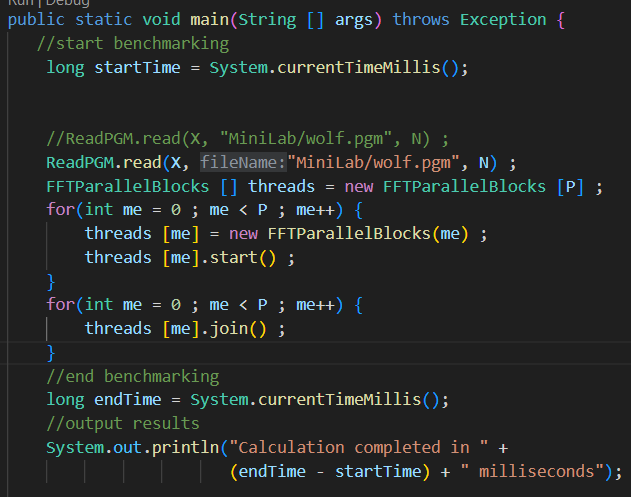
\includegraphics[width=0.9\columnwidth]{Figures/Report/2.png}
    \caption{Screenshot Parallel FFT main method }
    \label{fig:rep-2}
\end{figure}

The rest of the FFTImage main method resides in the new run method in the parallel version. 
As most of the calculations are in-place in the original, each thread created its own temporary local copy or 'CRe' and 'CIm' to process \autoref{fig:rep-3}.
\begin{figure}[H] 
    \centering
    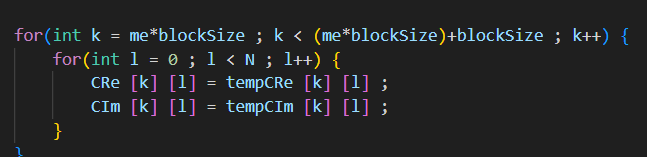
\includegraphics[width=0.9\columnwidth]{Figures/Report/4.png}
    \caption{Screenshot Parallel FFT temporary variable}
    \label{fig:rep-3}
\end{figure}

Once the pixel values are calculated, the threads are synchronised using 'java.util.concurrent.CyclicBarrier', the threads update the now static shared variables, shown in \autoref{fig:rep-1}.
\begin{figure}[H] 
    \centering
    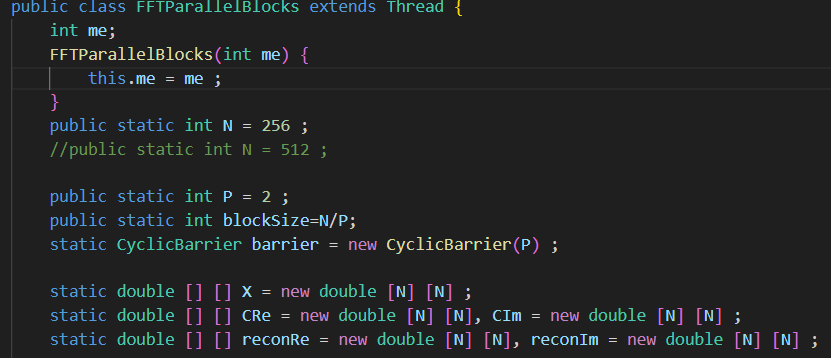
\includegraphics[width=0.9\columnwidth]{Figures/Report/1.png}
    \caption{Screenshot Parallel FFT Shared Variables }
    \label{fig:rep-1}
\end{figure}
Conditional statements are used to ensure graphical outputs are only executed by a single thread. Both programs were run using the original 'wolf.pgm' image along with a larger 512x512 image.

For both images, each program was run three times to ensure accuracy.
The parallel version was run with 2, 4 and 8 threads.

\section{Results}

\autoref{tab:minLab-512} shows the results for the large image experiment, the data is also graphed in \autoref{fig:miniLab-graph-512}. The fastest parallel speedup achieved in this case is two threaded version: $948/1076 = 0.88104089219$. This is an increase in execution time compared to the sequential program. The parallel efficiency for this is $0.88104089219 / 2 = 0.44052044609$ or 44\%, a significant decrease in performance.


\begin{table}[htbp]
        \centering
        \begin{tabular}{|c|c|c|c|c|}
        \hline
        \textbf{Number of threads} & \textbf{1} & \textbf{2} & \textbf{4} & \textbf{8} \\
        \hline
        Run 1 (ms) & 948 & 1274 & 1322 & 1594 \\
        \hline
        Run 2 (ms) & 1092 & 1290 & 1198 & 1683 \\
        \hline
        Run 3 (ms) & 1232 & 1076 & 1268 & 1494 \\
        \hline
        Mean Average (ms) & 1091 & 1213 & 1263 & 1590 \\
        \hline
        
                                  
        \end{tabular}
        \caption{FFT Parallel Benchmarking N = 512}
        \label{tab:minLab-512}
\end{table}  
\begin{figure}[H] 
    \centering
    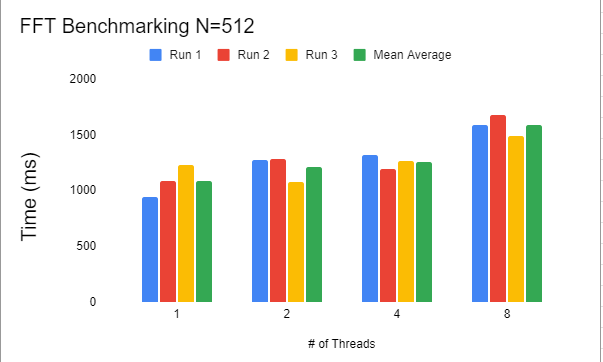
\includegraphics[width=0.9\columnwidth]{Figures/Report/graph 512.png}
    \caption{FFT Parallel benchmarking results graph N = 512 }
    \label{fig:miniLab-graph-512}
\end{figure}
   

\autoref{tab:minLab-256} shows the results for the small image experiment, the data is also graphed in \autoref{fig:miniLab-graph-256}. The fastest parallel speedup achieved in this case is eight threaded version: $687/790 = 0.86962025316$. This is an increase in execution time compared to the sequential program. The parallel efficiency for this is $0.86962025316 / 8 = 0.10870253164$ or 11\%.

\begin{table}[htbp]
      \centering
      \begin{tabular}{|c|c|c|c|c|}
\hline
\textbf{Number of threads} & \textbf{1} & \textbf{2} & \textbf{4} & \textbf{8} \\
\hline
Run 1 & 802 &842	&918	&937 \\
\hline
Run 2 & 687 &826	&845	&790 \\
\hline
Run 3 & 1081    &794	&852	&1011 \\
\hline
Mean Average &  857 &821	&872	&913 \\
\hline
      \end{tabular}
      \caption{FFT Parallel Benchmarking N = 256}
      \label{tab:minLab-256}
    \end{table}  
\begin{figure}[H] 
    \centering
    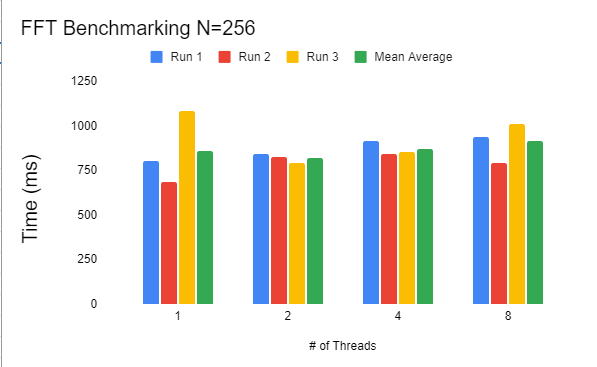
\includegraphics[width=0.9\columnwidth]{Figures/Report/graph 256.png}
    \caption{FFT Parallel benchmarking results graph N = 256 }
    \label{fig:miniLab-graph-256}
\end{figure}
   


\section{Conclusion}
The parallel implementation was unsuccessful in decreasing the execution time of the original sequential program. Perhaps with increased problem size the parallel speedup would increase. 
